% ******************************************************** %
%              TEMPLATE DE INFORME ORGA2 v0.1              %
% ******************************************************** %
% ******************************************************** %
%                                                          %
% ALGUNOS PAQUETES REQUERIDOS (EN UBUNTU):                 %
% ========================================
%                                                          %
% texlive-latex-base                                       %
% texlive-latex-recommended                                %
% texlive-fonts-recommended                                %
% texlive-latex-extra?                                     %
% texlive-lang-spanish (en ubuntu 13.10)                   %
% ******************************************************** %


\documentclass[a4paper]{article}
\usepackage[spanish]{babel}
\usepackage[utf8]{inputenc}
\usepackage{charter}   % tipografia
\usepackage{graphicx}
%\usepackage{makeidx}
\usepackage{paralist} %itemize inline

%\usepackage{float}
%\usepackage{amsmath, amsthm, amssymb}
%\usepackage{amsfonts}
%\usepackage{sectsty}
%\usepackage{charter}
%\usepackage{wrapfig}
\usepackage{listings}
\lstset{language=C}
\usepackage{caption}
\usepackage{color}

% \setcounter{secnumdepth}{2}
\usepackage{underscore}
\usepackage{caratula}
\usepackage{url}
\usepackage[document]{ragged2e}
\usepackage[export]{adjustbox}
\usepackage{subcaption}
\usepackage{floatrow}


% ********************************************************* %
% ~~~~~~~~              Code snippets             ~~~~~~~~~ %
% ********************************************************* %

\usepackage{color} % para snipets de codigo coloreados
\usepackage{fancybox}  % para el sbox de los snipets de codigo

\definecolor{litegrey}{gray}{0.94}

\newenvironment{codesnippet}{%
	\begin{Sbox}\begin{minipage}{\textwidth}\sffamily\small}%
	{\end{minipage}\end{Sbox}%
		\begin{center}%
		\vspace{-0.4cm}\colorbox{litegrey}{\TheSbox}\end{center}\vspace{0.3cm}}



% ********************************************************* %
% ~~~~~~~~         Formato de las páginas         ~~~~~~~~~ %
% ********************************************************* %

\usepackage{fancyhdr}
\usepackage{parskip}
\pagestyle{fancy}

%\renewcommand{\chaptermark}[1]{\markboth{#1}{}}
\renewcommand{\sectionmark}[1]{\markright{\thesection\ - #1}}

\fancyhf{}

\fancyhead[LO]{Sección \rightmark} % \thesection\
\fancyfoot[LO]{\small{Nicolas Bukovits, Kevin Frachtenberg Goldsmit, Laura Muiño}}
\fancyfoot[RO]{\thepage}
\renewcommand{\headrulewidth}{0.5pt}
\renewcommand{\footrulewidth}{0.5pt}
\setlength{\hoffset}{-0.8in}
\setlength{\textwidth}{16cm}
%\setlength{\hoffset}{-1.1cm}
%\setlength{\textwidth}{16cm}
\setlength{\headsep}{0.5cm}
\setlength{\textheight}{25cm}
\setlength{\voffset}{-0.7in}
\setlength{\headwidth}{\textwidth}
\setlength{\headheight}{13.1pt}
\setlength{\parindent}{4em}
\setlength{\parskip}{\baselineskip}

\renewcommand{\baselinestretch}{1.1}  % line spacing

% ******************************************************** %


\begin{document}


\thispagestyle{empty}
\materia{Sistemas Operativos}
\submateria{Primer Cuatrimestre de 2018}
\titulo{Trabajo Práctico 2}
\subtitulo{Sistemas distribuidos}
\integrante{Nicolas Bukovits}{546/14}{nicko_buk@hotmail.com}
\integrante{Kevin Frachtenberg}{247/14}{kevinfra94@gmail.com}
\integrante{Laura Muiño}{399/11}{lauramuino2@gmail.com}
\maketitle

%{\small\textbf{\flushleft{Resumen}}\\
\abstract {En el siguiente trabajo pr\'actico, se realiz\'o una implementaci\'on de un protocolo de envío de mensajes entre procesos concurrentes. En el mismo se desarrolló un sistema de blockchain.

%\newpage

%\thispagestyle{empty}
%\vfill


\thispagestyle{empty}
\vspace{3cm}
\tableofcontents
\newpage


%\normalsize
\newpage



\section{Analisis del protocolo}
\subsection{¿Puede este protocolo producir dos o más blockchains que nunca converjan?}

EL protocolo puede producir dos o más blockchains que nunca converjan. Si se tienen dos nodos A y B que cuando B comunica a A que encontró un bloque nuevo, y si A, antes de recibir el mensaje de B, encontró un bloque nuevo con el mismo índice que el nuevo bloque de B, entonces cuando A reciba el mesaje de B, va a descartar su bloque porque va a apostar por su propia cadena. Este esquema se puede repetir una cantidad de veces indeterminadas generan dos bifurcaciones que nunca converjen.


\subsection{¿Cómo afecta la demora o la pérdida en la entrega de paquetes al protocolo?}

La demora en la entrega de paquetes puede producir dos bifuraciones como lo mencionado en la pregunta anterior. La pérdida de mensajes puede producir que un nodo quede lo suficientemente desactualizado como para que el indice de su último bloque esté a una distancia mayor que la máxima diferencia tolerada de bloques generando nuevamente una bifurcación que podría no converjer.  

\subsection{¿Cómo afecta el aumento o la disminución de la dificultad del Proof-of-Work a los conflictos entre nodos y a la convergencia?}

La variación de la dificultad de \textit{Proof-of-Work} está directamente relacionada con la convergencia del proceso de minar bloques, e inversamente con los conflictos producidos entre los nodos al competir por agregar bloques propios a la cadena. Es decir, a mayor dificultad, mayor el tiempo total del proceso y menor la cantidad de conflictos entre nodos.
\\
Al aumentar dicha dificultad, observamos que los procesos tardan más en encontrar un hash que cumpla las condiciones de validez, haciendo menos probable que dos nodos encuentren un hash para un bloque de mismo índice.
Todo lo contrario sucede si se disminuye la dificultad; el proceso tarda menos en llegar al tamaño máximo de la cadena y se producen más conflictos.

Para mostrar esto, se realizaron 40 ejecuciones con dificultad 8 y 15 (20 cada una), donde se buscaba alcanzar los 200 bloques en la cadena y la diferencia máxima aceptada entre cadenas era de 5 bloques. Los resultados obtenidos del experimento, se volcaron en el siguiente gráfico, el cual muestra la cantidad de conflictos promedio para cada dificultad.

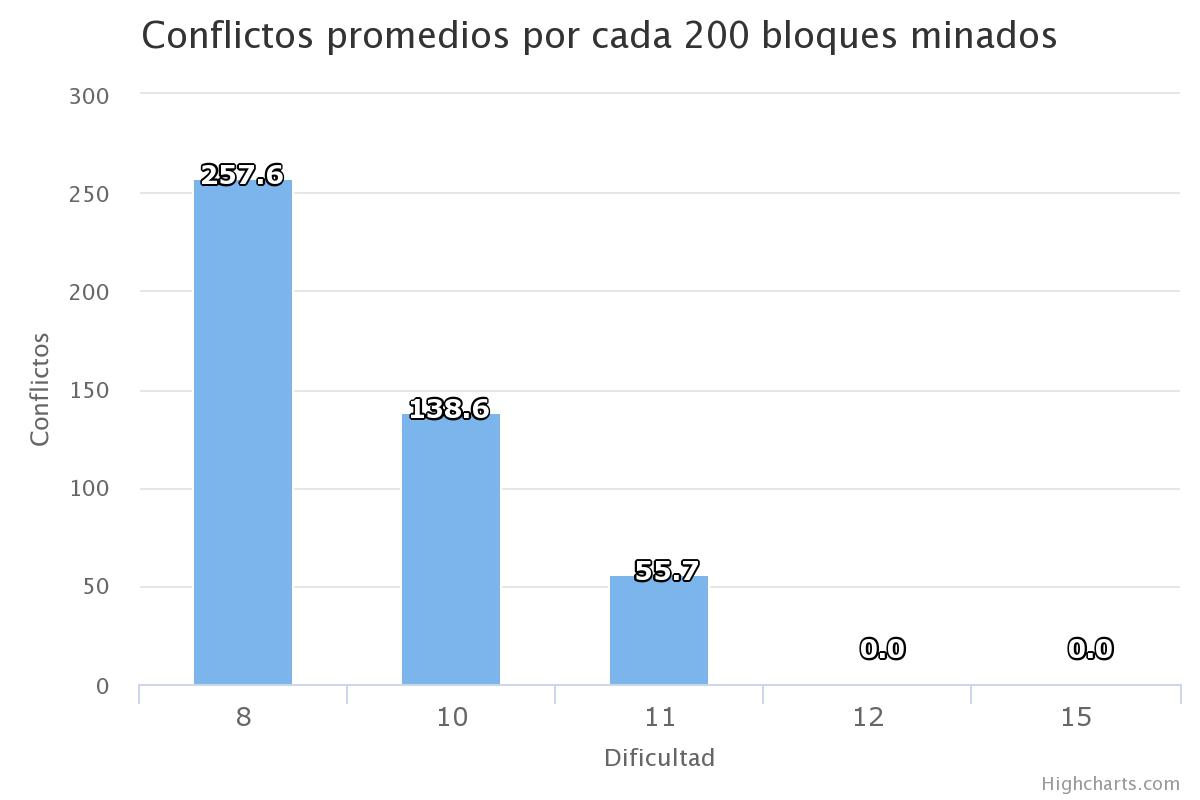
\includegraphics[scale=0.35]{imagenes/conflictos-promedio.jpeg}

\end{document}